\documentclass[conference]{IEEEtran}
\IEEEoverridecommandlockouts
\usepackage{cite}
\usepackage{amsmath,amssymb}
\usepackage{graphicx}
\usepackage{booktabs}
\usepackage{xcolor}
\usepackage{url}
\usepackage[hidelinks]{hyperref}
\graphicspath{{../docs/img/}}

\begin{document}

\title{Design and Verification of a Direct-Mapped Cache Controller in Verilog with Trace-Driven Performance Analysis\\
{\footnotesize Modern Computer Architecture --- Project~6, Phase~I}}

% ---------------- EDIT: replace placeholders with your group's details ----------------
\author{
\IEEEauthorblockN{Kartik Madaan}
\IEEEauthorblockA{B.Tech CS \& AI\\ \textit{[University Name]}}
\and
\IEEEauthorblockN{[Member 2]}
\IEEEauthorblockA{B.Tech CS \& AI\\ \textit{[University Name]}}
\and
\IEEEauthorblockN{[Member 3]}
\IEEEauthorblockA{B.Tech CS \& AI\\ \textit{[University Name]}}
\and
\IEEEauthorblockN{[Member 4]}
\IEEEauthorblockA{B.Tech CS \& AI\\ \textit{[University Name]}}
\and
\IEEEauthorblockN{[Member 5]}
\IEEEauthorblockA{B.Tech CS \& AI\\ \textit{[University Name]}}
}

\maketitle

% =====================================================================================
\begin{abstract}
The widening gap between processor and DRAM speed makes the cache the most important
component of the memory hierarchy. This paper presents the design, verification and
evaluation of a synthesizable direct-mapped cache controller written in Verilog-2005. The
cache holds 1\,KB in 64 lines of 16-byte blocks, decodes 32-bit addresses into a 22-bit tag,
6-bit index and 4-bit offset, and is controlled by a four-state finite-state machine
implementing a read-allocate, write-through, no-write-allocate policy. A self-checking
directed testbench (16/16 checks passing) verifies cold, conflict and capacity behaviour,
write-through correctness and valid-bit reset. A trace-driven testbench runs seven
synthetic workloads and cross-checks every load value, every hit/miss decision and the total
cycle count against an independent Python reference model; all 28 runs over four cache
geometries match exactly. With a 10-cycle main memory, the cache achieves a 97.5\% hit rate
and a 5.22$\times$ speed-up on a loop-oriented workload and 2.40$\times$ on a streaming workload,
while pathological conflict patterns expose the main weakness of direct mapping.
Yosys/nextpnr synthesis reports 256 flip-flops and a post-route $F_{max}$ of 61.4\,MHz on a
Lattice ECP5 FPGA.
\end{abstract}

\begin{IEEEkeywords}
cache memory, direct-mapped cache, cache controller, FSM, Verilog, AMAT, memory hierarchy, FPGA
\end{IEEEkeywords}

% =====================================================================================
\section{Introduction}
Processor performance has improved far faster than DRAM latency for decades, a trend
described as the \emph{memory wall}~\cite{wulf1995}. A main-memory access now costs tens to
hundreds of processor cycles, so without a cache almost every load would stall the pipeline.
Caches exploit \emph{temporal} locality (recently used data is likely to be reused) and
\emph{spatial} locality (neighbouring data is likely to be used soon) by keeping a small,
fast copy of recently accessed blocks close to the processor~\cite{hp_quant,hp_cod}.

The simplest cache organization is the \emph{direct-mapped} cache, in which every memory
block can live in exactly one cache line selected by the index bits of its address. Its
single tag comparison gives the shortest hit time and the lowest hardware cost. Its
weakness is \emph{conflict misses}, which happen when two active blocks share an index.

This project implements such a cache controller at the register-transfer level, verifies it
with directed and trace-driven testbenches, and quantifies its behaviour with hit rate,
average memory access time (AMAT), speed-up over a cache-less baseline, memory traffic and
FPGA synthesis results. The contributions are:
\begin{itemize}
  \item a parameterised, synthesizable Verilog cache controller (size, block size) with a
        clear datapath/controller split and built-in performance counters;
  \item a two-level verification strategy: directed self-checking tests plus trace-driven
        tests checked access-by-access against a Python reference model;
  \item a quantitative study over seven workloads and sweeps of cache size, block size and
        memory latency, compared against a no-cache baseline.
\end{itemize}

% =====================================================================================
\section{Literature Review}
\textbf{Foundations.} Smith's survey~\cite{smith1982} established the vocabulary and
methodology still used today: placement, replacement and write policies, and
trace-driven simulation as the way to evaluate them. Hennessy and Patterson~\cite{hp_quant}
formalised the AMAT model,
$\text{AMAT} = t_{hit} + m \cdot t_{penalty}$,
and the ``3C'' classification of misses into compulsory, capacity and conflict misses.
This paper uses both directly.

\textbf{Direct-mapped vs.\ associative.} Hill~\cite{hill1988} argued that, despite higher miss rates,
direct-mapped caches can deliver \emph{lower} effective access time because their hit path
avoids way-selection multiplexers and can be made faster and larger. Hill and
Smith~\cite{hill1989} quantified the miss-rate gap: going from direct-mapped to 2-way
associativity removes a large share of conflict misses, and returns diminish at higher
associativity. Przybylski \emph{et al.}~\cite{przybylski1988,przybylski1990} showed that cache
organisation must be co-optimised with cycle time, because a design that minimises miss rate
alone can lose overall performance.

\textbf{Reducing conflict misses.} Jouppi~\cite{jouppi1990} kept the fast direct-mapped hit
path and recovered most conflict misses with a small fully-associative \emph{victim cache}
and \emph{stream buffers} for prefetching. Lam \emph{et al.}~\cite{lam1991} showed that
software, through array padding and blocking (tiling), can remove self- and cross-interference
in numerical kernels. Our \texttt{vecadd} experiment reproduces this effect.

\textbf{Write policies.} Goodman~\cite{goodman1983} analysed how caches reduce
processor--memory traffic and the trade-off between write-through and write-back.
Write-through keeps memory consistent and simplifies the controller at the cost of more write
traffic. It is commonly paired with no-write-allocate~\cite{hp_cod}, which is the combination
chosen here. Write-back is left for a later phase (Project~8).

\textbf{Open hardware tool flows.} Icarus Verilog~\cite{icarus}, GTKWave, Yosys~\cite{yosys}
and nextpnr~\cite{nextpnr} make a complete RTL-to-timing flow possible without vendor
tools. This project uses that flow.

% =====================================================================================
\section{Proposed Solution}

\subsection{Cache organisation and address mapping}
The cache parameters are: capacity $C = 1024$\,B, block size $B = 16$\,B,
$N = C/B = 64$ lines and 32-bit byte addresses, so
\begin{equation}
\underbrace{a[31{:}10]}_{\text{tag, 22 b}}\;|\;\underbrace{a[9{:}4]}_{\text{index, 6 b}}\;|\;
\underbrace{a[3{:}0]}_{\text{offset, 4 b}}
\end{equation}
Offset bits $a[3{:}2]$ select one of four 32-bit words in the block. Each line stores
1 valid bit, a 22-bit tag and 128 data bits. All widths come from the \texttt{CACHE\_BYTES}
and \texttt{BLOCK\_BYTES} parameters with \texttt{\$clog2}, so other geometries need no code
changes. Four geometries were verified (Section~\ref{sec:results}).

\begin{figure*}[!t]
\centering
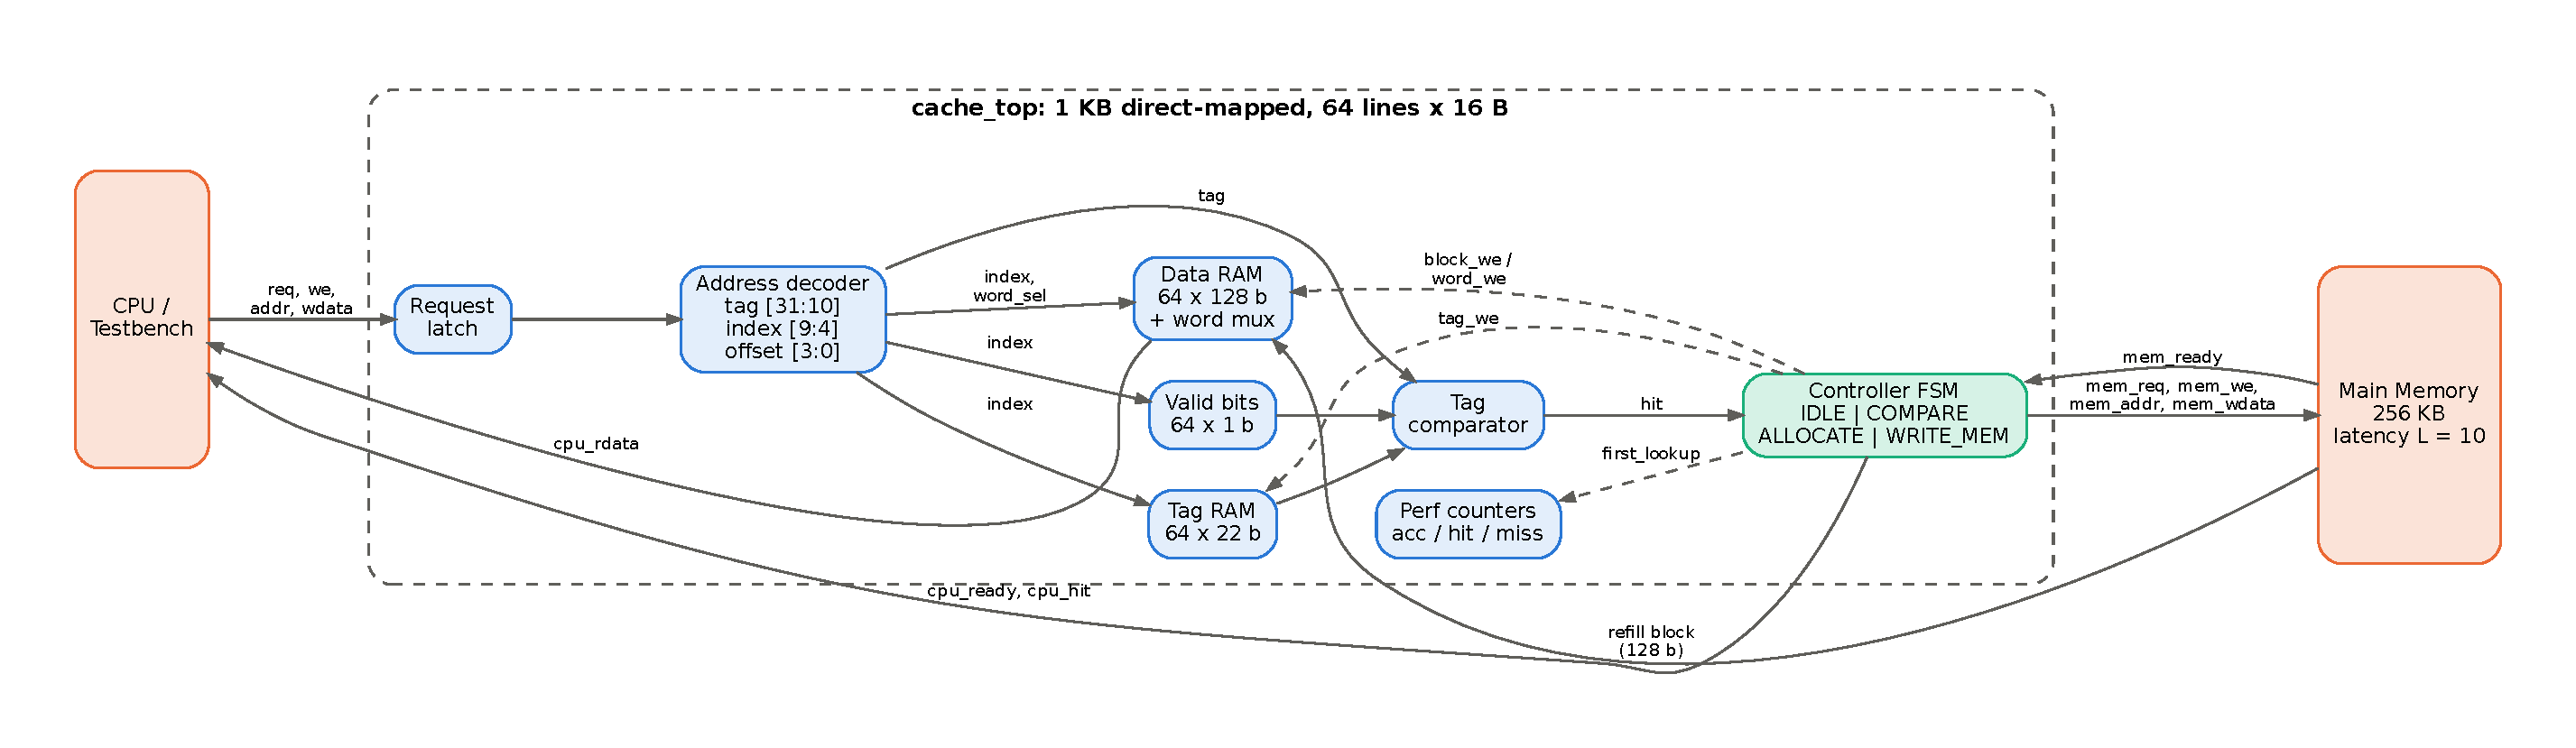
\includegraphics[width=0.92\textwidth]{block_diagram.pdf}
\caption{Block diagram of the direct-mapped cache (\texttt{cache\_top}). Solid lines are data
paths, dashed lines are control strobes from the FSM.}
\label{fig:block}
\end{figure*}

\subsection{Datapath}
Fig.~\ref{fig:block} shows the module hierarchy. The modules are:
\begin{itemize}
  \item \textbf{Request latch}: registers \texttt{cpu\_addr}, \texttt{cpu\_wdata} and
        \texttt{cpu\_we} when a request is accepted, so the CPU may change its inputs.
  \item \textbf{\texttt{addr\_decoder}}: purely combinational split into tag, index, offset
        and word select.
  \item \textbf{\texttt{tag\_ram}} ($64\times22$\,b) and \textbf{\texttt{data\_ram}}
        ($64\times128$\,b): synchronous write and asynchronous read. The data RAM has a
        full-block write port for refills and a single-word write port for store hits.
  \item \textbf{\texttt{valid\_ram}}: a 64-bit flip-flop vector, so one reset cycle
        invalidates the whole cache.
  \item \textbf{\texttt{tag\_comparator}}: $\textit{hit} = V \land (\textit{tag}_{req} = \textit{tag}_{stored})$.
  \item \textbf{Performance counters}: accesses, hits and misses, incremented only on the
        \emph{first} lookup of each request, so the re-lookup after a refill is not counted
        twice.
\end{itemize}

\subsection{Controller FSM}
Fig.~\ref{fig:fsm} shows the controller. In \textsc{Idle} it waits for \texttt{cpu\_req}
and latches the request. In \textsc{Compare} it performs the lookup:
\begin{itemize}
  \item a load hit returns data and asserts \texttt{cpu\_ready};
  \item a load miss moves to \textsc{Allocate}, which holds \texttt{mem\_req} until
        \texttt{mem\_ready}, writes the 128-bit block, tag and valid bit, and returns to
        \textsc{Compare}, where the access now hits;
  \item any store moves to \textsc{Write\_Mem}, which writes the word through to memory; on
        a store hit the cached word is updated in the same cycle, so cache and memory never
        disagree.
\end{itemize}

\begin{figure}[!t]
\centering
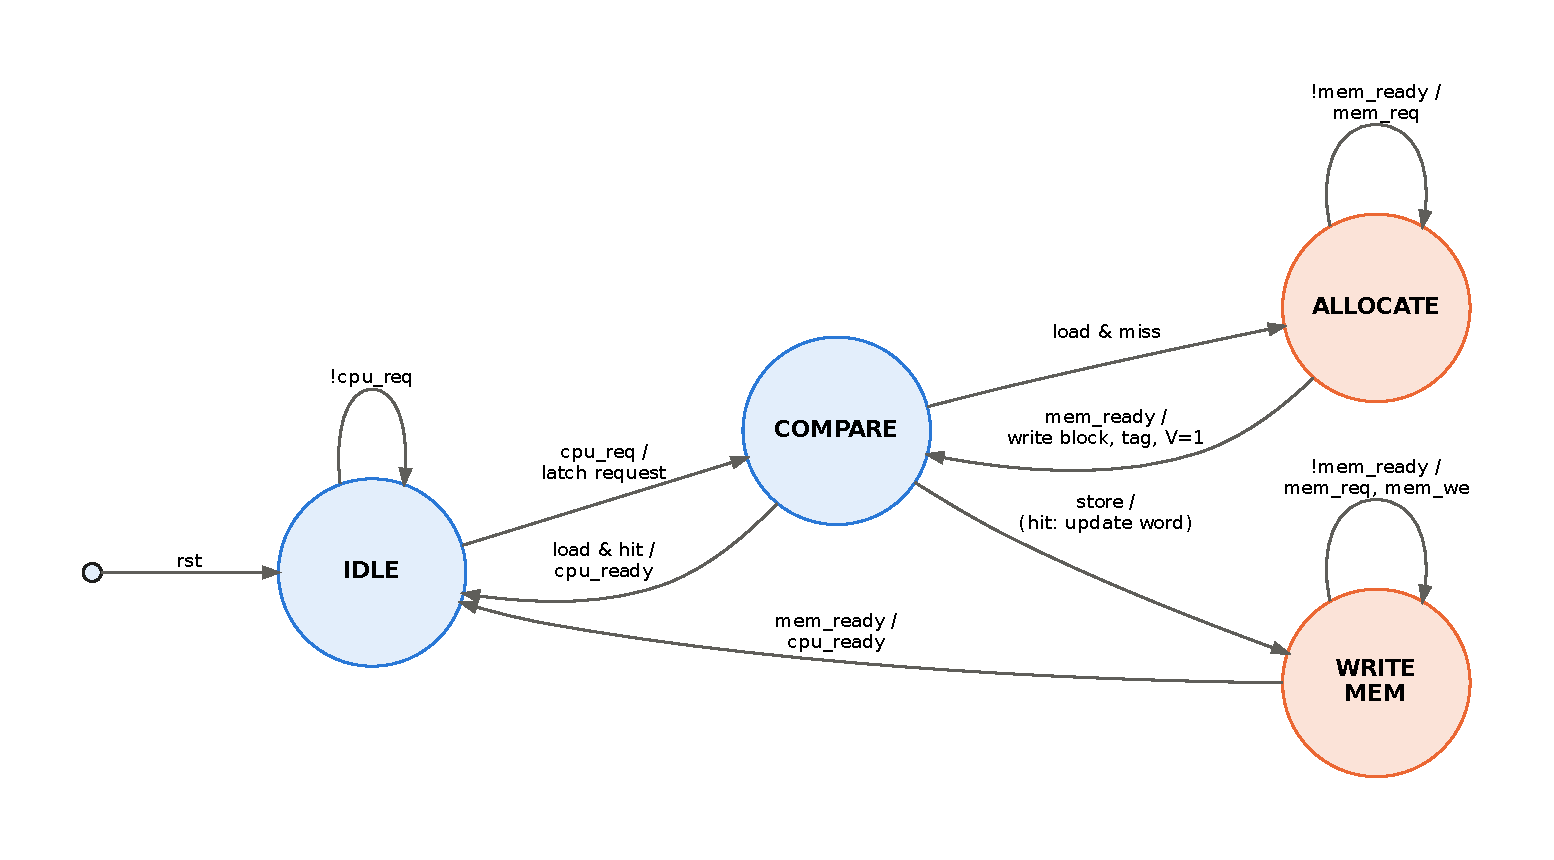
\includegraphics[width=\columnwidth]{fsm.pdf}
\caption{Cache-controller FSM (read-allocate, write-through, no-write-allocate).}
\label{fig:fsm}
\end{figure}

\subsection{Timing model}
With main-memory latency $L$, the cycle costs (verified in simulation) are:
\begin{itemize}
  \item load hit: 2 cycles (\textsc{Idle}+\textsc{Compare});
  \item load miss: $L+4$ cycles;
  \item store: $L+3$ cycles;
  \item no-cache baseline: $L+2$ cycles for every access.
\end{itemize}
The load miss penalty is therefore $t_{penalty}=L+2$ and
\begin{equation}
\text{AMAT}_{load} = 2 + m_{load}\,(L+2).
\end{equation}

\subsection{Verification methodology}
\textbf{Directed testbench} (\texttt{tb\_directed.v}). Sixteen self-checking checks cover:
\begin{itemize}
  \item a cold miss and its latency;
  \item temporal and spatial hits and the hit latency;
  \item a conflict miss followed by eviction (0x440 and 0x040 share index~4);
  \item a write hit, checked in both cache and main memory;
  \item a write miss without allocation;
  \item filling and re-reading all 64 lines;
  \item invalidation on reset.
\end{itemize}

\textbf{Trace-driven testbench} (\texttt{tb\_trace.v}). It replays a trace and keeps a shadow
copy of memory. It checks (i) every load value against the shadow and (ii) every hit/miss
decision against the expected sequence produced by an independent Python model
(\texttt{cache\_model.py}). The same traces are also run on a no-cache baseline with the same
interface (\texttt{nocache\_top.v}).

The seven workloads are:
\begin{itemize}
  \item \emph{sequential}: an 8\,KB stream;
  \item \emph{loop}: 10 passes over 512\,B;
  \item \emph{random}: random reads over 64\,KB;
  \item \emph{conflict}: alternating A and A+1\,KB;
  \item \emph{vecadd}: $C[i]=A[i]+B[i]$, with the arrays either 16\,KB-aligned or padded by
        256\,B;
  \item \emph{mixed}: 70\% hot set, 30\% random, 20\% stores.
\end{itemize}

% =====================================================================================
\section{Results and Analysis}\label{sec:results}

\subsection{Functional verification}
All 16 directed checks pass. Fig.~\ref{fig:wave} shows a cold miss: the FSM stays in
\textsc{Allocate} for $L+1$ cycles, writes the block when \texttt{mem\_ready} pulses, re-enters
\textsc{Compare} with \texttt{hit}=1 and returns \texttt{0xC0DE0010}. The next three requests to
the same block hit in 2 cycles each. Across the 1\,KB/16\,B design point and three further
geometries (512\,B/16\,B, 2\,KB/32\,B, 1\,KB/4\,B), \textbf{28 of 28} trace runs agree exactly
with the reference model in data, per-access hit/miss decision and total cycle count, with zero
data errors.

\begin{figure*}[!t]
\centering
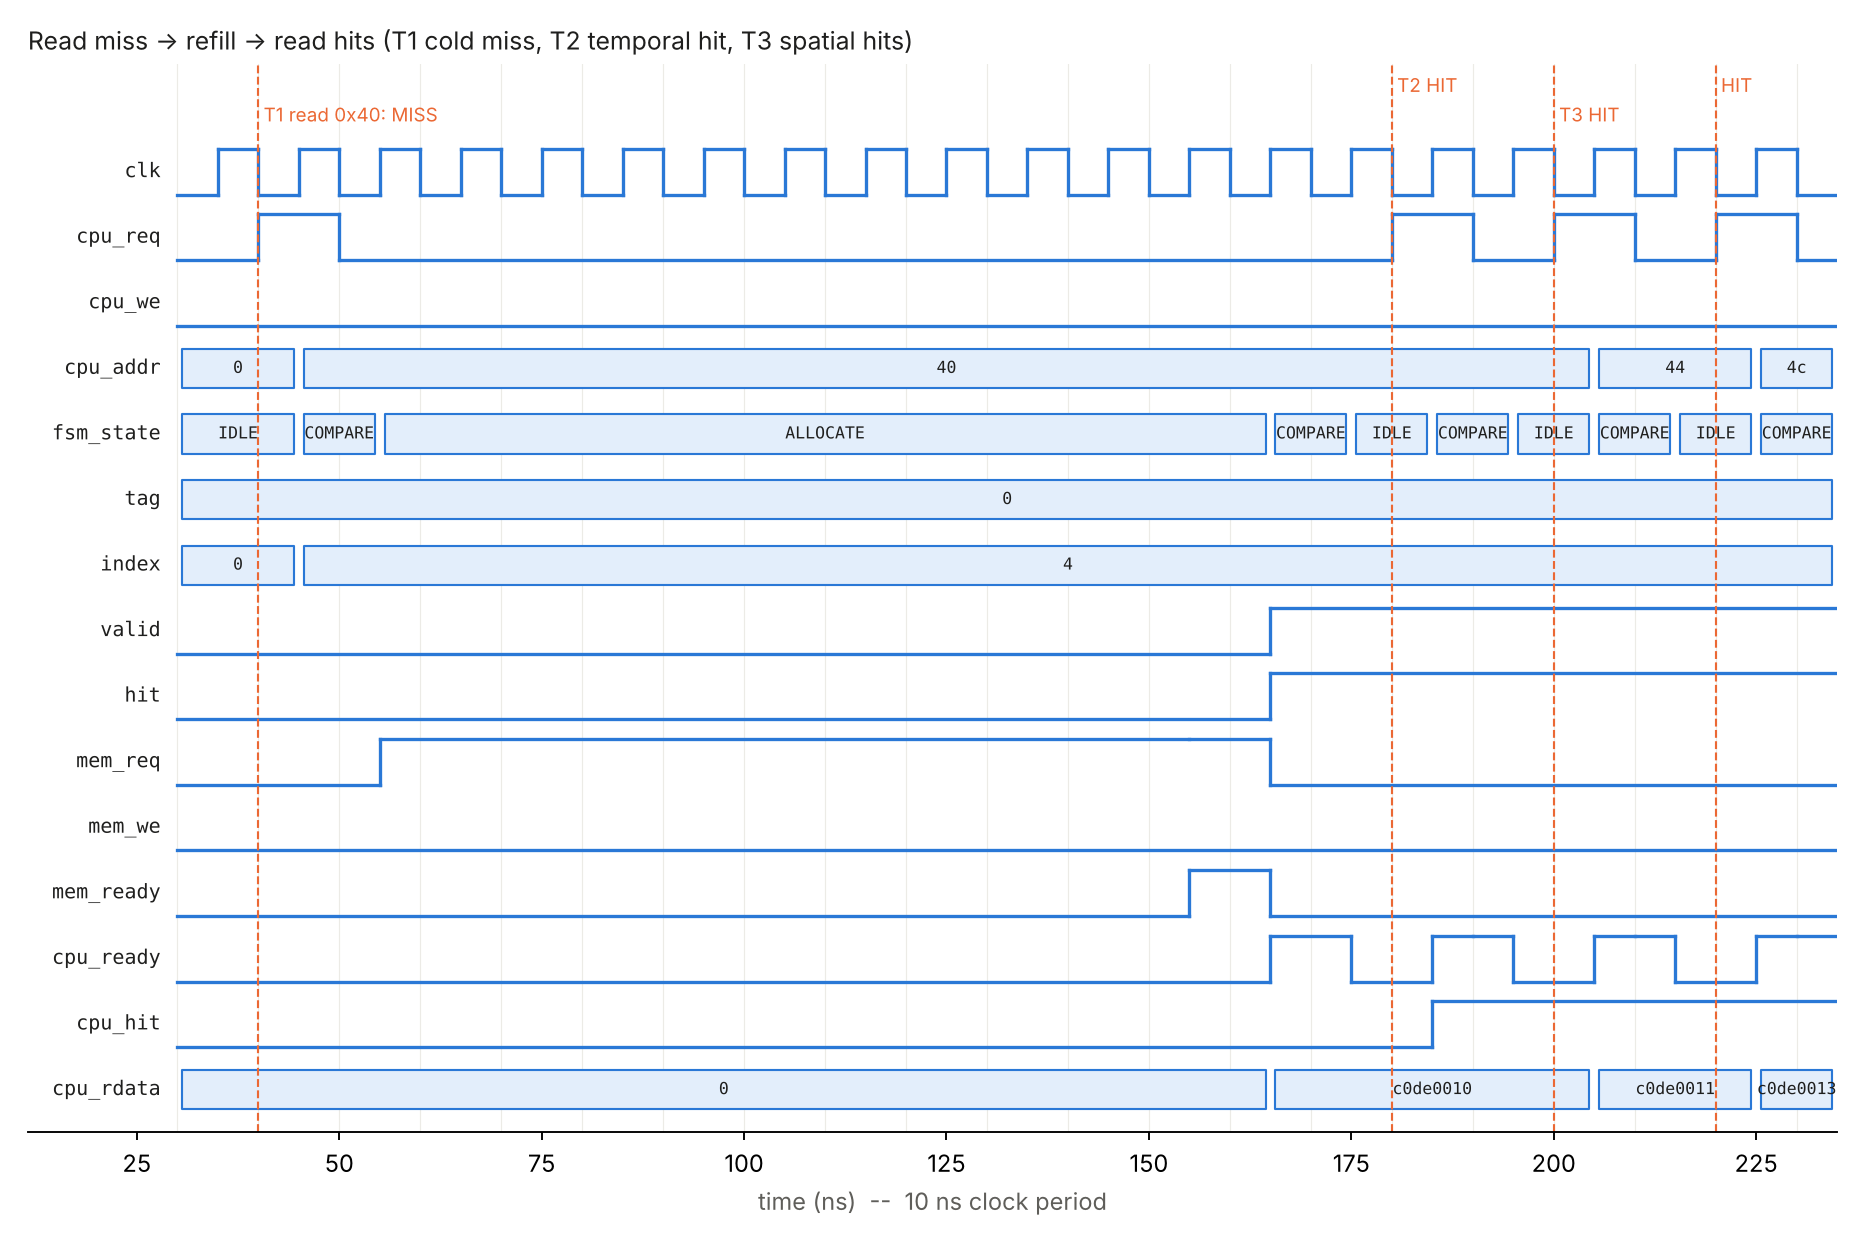
\includegraphics[width=0.85\textwidth]{wave_miss_refill_hit.png}
\caption{Simulation waveform (rendered from the Icarus Verilog VCD): cold miss
$\rightarrow$ refill $\rightarrow$ temporal and spatial hits.}
\label{fig:wave}
\end{figure*}

\begin{table}[!t]
\centering
\caption{RTL results: 1\,KB direct-mapped cache, 16\,B blocks, $L=10$ cycles}
\label{tab:results}
\setlength{\tabcolsep}{3pt}
\begin{tabular}{lrrrrrr}
\hline
Trace & Acc. & Hit & AMAT & Cycles & Cycles & Speed- \\
 & & rate & (load) & cache & no cache & up \\
\hline
sequential & 2048 & 75.0\% & 5.00 & 10240 & 24576 & 2.40$\times$ \\
loop & 1280 & 97.5\% & 2.30 & 2944 & 15360 & 5.22$\times$ \\
random & 2000 & 1.1\% & 13.87 & 27736 & 24000 & 0.87$\times$ \\
conflict & 1000 & 0.0\% & 14.00 & 14000 & 12000 & 0.86$\times$ \\
vecadd (aligned) & 1536 & 0.0\% & 14.00 & 20992 & 18432 & 0.88$\times$ \\
vecadd (padded) & 1536 & 50.0\% & 5.00 & 11776 & 18432 & 1.57$\times$ \\
mixed & 3000 & 57.8\% & 7.03 & 25042 & 36000 & 1.44$\times$ \\
\hline
\end{tabular}
\end{table}


\subsection{Performance}
Table~\ref{tab:results} and Fig.~\ref{fig:bars} summarise the main design point.

\textbf{Loop.} The 512\,B working set fits in the cache, so only the 32 compulsory misses
remain. This gives a 97.5\% hit rate, $\text{AMAT}=2.30$ cycles and a \textbf{5.22$\times$}
speed-up, and memory traffic falls from 1280 to 32 transactions.

\textbf{Sequential.} The stream has no reuse, but each refill brings in four words, so the
hit rate is exactly $1-1/4=75\%$. This gives $\text{AMAT}=5.0$ and a 2.40$\times$ speed-up.

\textbf{Random and conflict.} These show the cost of a cache without locality. Every miss
pays two extra cycles over the baseline, so the cache is about 13\% \emph{slower}.

\textbf{vecadd.} This workload shows conflict misses most clearly. With 16\,KB-aligned
arrays, $A[i]$ and $B[i]$ map to the same line and evict each other on every access, giving a
0\% hit rate. Padding $B$ by 256\,B removes the conflict: the load miss rate drops from 100\%
to 25\% and the kernel becomes 1.57$\times$ faster than the baseline. This is the effect
reported by Lam \emph{et al.}~\cite{lam1991} and the motivation for victim
caches~\cite{jouppi1990} and set-associativity~\cite{hill1989}.

\begin{figure}[!t]
\centering
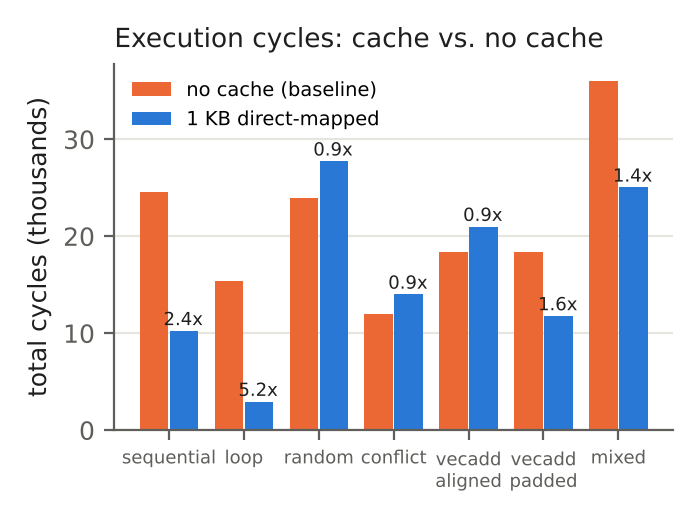
\includegraphics[width=\columnwidth]{speedup_bars.png}
\caption{Total execution cycles with and without the cache ($L=10$); labels show speed-up.}
\label{fig:bars}
\end{figure}

\subsection{Design-space exploration}
Using the validated model, Fig.~\ref{fig:sweep} sweeps cache size and block size.

\textbf{Cache size.} The \emph{mixed} hit rate rises from 24.6\% at 256\,B to 57.8\% at 1\,KB
and 67.3\% at 8\,KB, with diminishing returns once the hot set fits. The \emph{loop} curve
saturates at 512\,B, its working-set size.

\textbf{Block size.} Larger blocks raise the \emph{sequential} hit rate from 0\% (4\,B) to
93.8\% (64\,B) because of spatial locality. This sweep assumes a block-wide memory bus with a
fixed miss penalty; on a narrower bus the penalty would grow with block size.

\textbf{Memory latency.} The benefit of the cache grows with latency: at $L=100$ the loop
speed-up reaches 22.4$\times$.

\begin{figure}[!t]
\centering
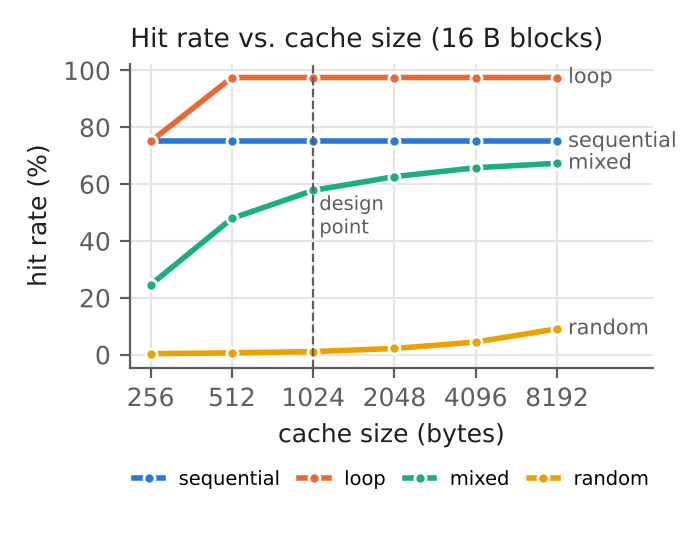
\includegraphics[width=\columnwidth]{sweep_cache_size.png}\\[2pt]
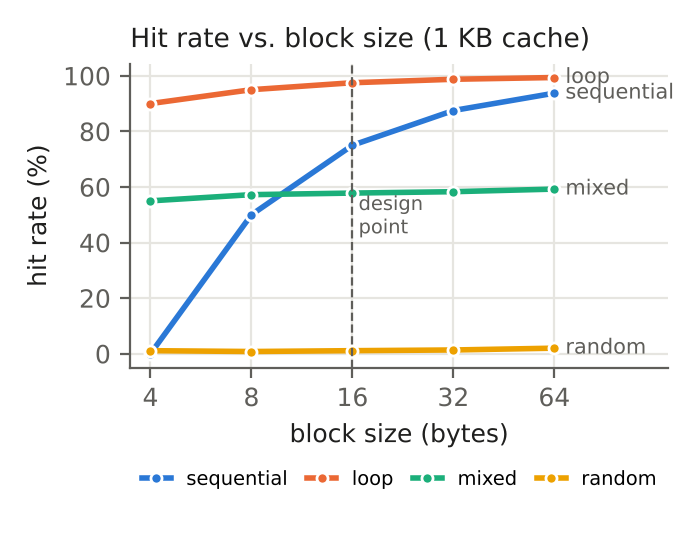
\includegraphics[width=\columnwidth]{sweep_block_size.png}
\caption{Hit rate vs.\ cache size (top) and block size (bottom); dashed line marks the
implemented design point.}
\label{fig:sweep}
\end{figure}

\subsection{Synthesis}
\texttt{cache\_top} was synthesised with Yosys~0.33 for two targets:
\begin{itemize}
  \item \textbf{Xilinx 7-series:} 321 logic LUTs, 233 FFs, 136 RAM64M LUT-RAM primitives
        (the asynchronous-read arrays map to distributed RAM) and no block RAM.
  \item \textbf{Lattice ECP5-85F, placed and routed out-of-context with nextpnr:} 4387 LUT4
        (5\%), 256 FFs, 512 distributed-RAM slices and one DP16KD block RAM.
\end{itemize}
The post-route \textbf{$F_{max}$ is 61.4\,MHz}. The critical path is tag-RAM read
$\rightarrow$ 22-bit compare $\rightarrow$ FSM next-state $\rightarrow$ array write enable,
which is the single-cycle \textsc{Compare} lookup.

% =====================================================================================
\section{Conclusion and Future Work}
We designed and verified a parameterised direct-mapped cache controller. Directed tests
and access-by-access agreement with a reference model over 28 runs establish its
correctness. The cache gives up to 5.22$\times$ speed-up and 40$\times$ less memory traffic
on workloads with locality. The conflict and \texttt{vecadd} experiments quantify the main
limitation of direct mapping.

Phase~II will:
\begin{itemize}
  \item add a 2-way set-associative variant with LRU replacement for a like-for-like
        comparison;
  \item add a write buffer or write-back policy to cut the $L+3$ store cost;
  \item pipeline the lookup with synchronous-read block RAM to raise $F_{max}$;
  \item deploy on an FPGA board with a Vivado timing report.
\end{itemize}

% =====================================================================================
\section*{Individual Contributions}
% ---------------- EDIT: make these match what each member actually did ----------------
\begin{itemize}
  \item \textbf{Kartik Madaan}: [describe actual contribution].
  \item \textbf{[Member 2]}: [describe actual contribution].
  \item \textbf{[Member 3]}: [describe actual contribution].
  \item \textbf{[Member 4]}: [describe actual contribution].
  \item \textbf{[Member 5]}: [describe actual contribution].
\end{itemize}

\section*{Artefacts}
Source code, testbenches, traces, scripts and synthesis logs:
\url{https://github.com/[username]/mca-project6-dm-cache}.\\
Prototype video: \url{[video link]}.

% =====================================================================================
\begin{thebibliography}{99}
\bibitem{hp_quant} J.~L.~Hennessy and D.~A.~Patterson, \emph{Computer Architecture: A Quantitative Approach}, 6th~ed. Cambridge, MA, USA: Morgan Kaufmann, 2017.
\bibitem{hp_cod} D.~A.~Patterson and J.~L.~Hennessy, \emph{Computer Organization and Design RISC-V Edition: The Hardware/Software Interface}, 2nd~ed. Morgan Kaufmann, 2020.
\bibitem{smith1982} A.~J.~Smith, ``Cache memories,'' \emph{ACM Computing Surveys}, vol.~14, no.~3, pp.~473--530, Sep.~1982.
\bibitem{hill1988} M.~D.~Hill, ``A case for direct-mapped caches,'' \emph{IEEE Computer}, vol.~21, no.~12, pp.~25--40, Dec.~1988.
\bibitem{hill1989} M.~D.~Hill and A.~J.~Smith, ``Evaluating associativity in CPU caches,'' \emph{IEEE Trans. Computers}, vol.~38, no.~12, pp.~1612--1630, Dec.~1989.
\bibitem{przybylski1988} S.~Przybylski, M.~Horowitz, and J.~Hennessy, ``Performance tradeoffs in cache design,'' in \emph{Proc. 15th Annu. Int. Symp. Computer Architecture (ISCA)}, 1988, pp.~290--298.
\bibitem{przybylski1990} S.~A.~Przybylski, \emph{Cache and Memory Hierarchy Design: A Performance-Directed Approach}. San Mateo, CA, USA: Morgan Kaufmann, 1990.
\bibitem{jouppi1990} N.~P.~Jouppi, ``Improving direct-mapped cache performance by the addition of a small fully-associative cache and prefetch buffers,'' in \emph{Proc. 17th Annu. Int. Symp. Computer Architecture (ISCA)}, 1990, pp.~364--373.
\bibitem{lam1991} M.~S.~Lam, E.~E.~Rothberg, and M.~E.~Wolf, ``The cache performance and optimizations of blocked algorithms,'' in \emph{Proc. ASPLOS-IV}, 1991, pp.~63--74.
\bibitem{goodman1983} J.~R.~Goodman, ``Using cache memory to reduce processor-memory traffic,'' in \emph{Proc. 10th Annu. Int. Symp. Computer Architecture (ISCA)}, 1983, pp.~124--131.
\bibitem{wulf1995} W.~A.~Wulf and S.~A.~McKee, ``Hitting the memory wall: Implications of the obvious,'' \emph{ACM SIGARCH Computer Architecture News}, vol.~23, no.~1, pp.~20--24, Mar.~1995.
\bibitem{verilog} \emph{IEEE Standard for Verilog Hardware Description Language}, IEEE Std 1364-2005, 2006.
\bibitem{icarus} S.~Williams, ``Icarus Verilog.'' [Online]. Available: \url{https://steveicarus.github.io/iverilog/}
\bibitem{yosys} C.~Wolf, ``Yosys Open SYnthesis Suite.'' [Online]. Available: \url{https://yosyshq.net/yosys/}
\bibitem{nextpnr} D.~Shah \emph{et al.}, ``Yosys+nextpnr: An open source framework from Verilog to bitstream for commercial FPGAs,'' in \emph{Proc. IEEE FCCM}, 2019, pp.~1--4.
\end{thebibliography}

\end{document}
